\documentclass[anon]{colt2020} % Anonymized submission
% \documentclass{colt2020} % Include author names

% The following packages will be automatically loaded:
% amsmath, amssymb, natbib, graphicx, url, algorithm2e

\title[Embedding dimension]{Embedding Dimension of Polyhedral Losses}
\usepackage{times}

\usepackage{lmodern}
\usepackage{hyperref}       % hyperlinks  %[implicit=false, bookmarks=false]
\usepackage{booktabs}       % professional-quality tables
\usepackage{amsfonts}       % blackboard math symbols
\usepackage{nicefrac}       % compact symbols for 1/2, etc.
\usepackage{microtype}      % microtypography

\usepackage{mathtools, verbatim}
%\usepackage[thmmarks, thref, amsthm]{ntheorem}
\usepackage{color}
\definecolor{darkblue}{rgb}{0.0,0.0,0.2}
\hypersetup{colorlinks,breaklinks,
	linkcolor=darkblue,urlcolor=darkblue,
	anchorcolor=darkblue,citecolor=darkblue}
\usepackage{wrapfig}
\usepackage{subcaption}
\usepackage[colorinlistoftodos,textsize=tiny]{todonotes} % need xargs for below
%\usepackage{accents}
\usepackage{bbm}
\usepackage{xspace}

%\usetikzlibrary{calc}
\newcommand{\Comments}{1}
\newcommand{\mynote}[2]{\ifnum\Comments=1\textcolor{#1}{#2}\fi}
\newcommand{\mytodo}[2]{\ifnum\Comments=1%
	\todo[linecolor=#1!80!black,backgroundcolor=#1,bordercolor=#1!80!black]{#2}\fi}
\newcommand{\raf}[1]{\mynote{green}{[RF: #1]}}
\newcommand{\raft}[1]{\mytodo{green!20!white}{RF: #1}}
\newcommand{\jessie}[1]{\mynote{purple}{[JF: #1]}}
\newcommand{\jessiet}[1]{\mytodo{purple!20!white}{JF: #1}}
\newcommand{\bo}[1]{\mynote{blue}{[Bo: #1]}}
\newcommand{\botodo}[1]{\mytodo{blue!20!white}{[Bo: #1]}}
\newcommand{\btw}[1]{\mytodo{orange!20!white}{BTW: #1}}
\ifnum\Comments=1               % fix margins for todonotes
\setlength{\marginparwidth}{1in}
\fi


\newcommand{\reals}{\mathbb{R}}
\newcommand{\posreals}{\reals_{>0}}%{\reals_{++}}
\newcommand{\nonnegreals}{\reals_{\geq 0}}%{\reals_{++}}
\newcommand{\dom}{\mathrm{dom}}
\newcommand{\epi}{\text{epi}}
\newcommand{\relint}{\mathrm{relint}}
\newcommand{\prop}[1]{\Gamma[#1]}
\newcommand{\eliccts}{\mathrm{elic}_\mathrm{cts}}
\newcommand{\eliccvx}{\mathrm{elic}_\mathrm{cvx}}
\newcommand{\elicpoly}{\mathrm{elic}_\mathrm{pcvx}}
\newcommand{\elicembed}{\mathrm{elic}_\mathrm{embed}}

\newcommand{\cell}{\mathrm{cell}}

\newcommand{\abstain}[1]{\mathrm{abstain}_{#1}}
\newcommand{\mode}{\mathrm{mode}}

\newcommand{\simplex}{\Delta_\Y}

% alphabetical order, by convention
\newcommand{\C}{\mathcal{C}}
\newcommand{\D}{\mathcal{D}}
\newcommand{\E}{\mathbb{E}}
\newcommand{\F}{\mathcal{F}}
\renewcommand{\H}{\mathcal{H}}
\newcommand{\N}{\mathcal{N}}
\newcommand{\I}{\mathcal{I}}
\newcommand{\R}{\mathcal{R}}
\newcommand{\T}{\mathcal{T}}
\newcommand{\U}{\mathcal{U}}
\newcommand{\V}{\mathcal{V}}
\newcommand{\X}{\mathcal{X}}
\newcommand{\Y}{\mathcal{Y}}
\renewcommand{\P}{\mathcal{P}}

\newcommand{\hinge}{L_{\mathrm{hinge}}}
\newcommand{\ellzo}{\ell_{\text{0-1}}}
\newcommand{\ellabs}[1]{\ell_{#1}}

\newcommand{\Opt}{\mathrm{Opt}}
\newcommand{\risk}[1]{\underline{#1}}
\newcommand{\inprod}[2]{\langle #1, #2 \rangle}%\mathrm{int}(#1)}
\newcommand{\inter}[1]{\mathrm{int}(#1)}%\mathrm{int}(#1)}
%\newcommand{\expectedv}[3]{\overline{#1}(#2,#3)}
\newcommand{\expectedv}[3]{\E_{Y\sim{#3}} {#1}(#2,Y)}
\newcommand{\toto}{\rightrightarrows}
\newcommand{\strip}{\mathrm{strip}}
\newcommand{\trim}{\mathrm{trim}}
\newcommand{\fplc}{finite-piecewise-linear and convex\xspace} %xspace for use in text
\newcommand{\conv}{\mathrm{conv}}
\newcommand{\indopp}{\bar{\mathbbm{1}}}
\newcommand{\ones}{\mathbbm{1}}
\DeclarePairedDelimiter\ceil{\lceil}{\rceil}

\newcommand{\Ind}[1]{\mathbf{1}\{#1\}}

\DeclareMathOperator*{\argmax}{arg\,max}
\DeclareMathOperator*{\argmin}{arg\,min}
\DeclareMathOperator*{\arginf}{arg\,inf}
\DeclareMathOperator*{\sgn}{sgn}

%\newtheorem{theorem}{Theorem}
%\newtheorem{lemma}{Lemma}
%\newtheorem{proposition}{Proposition}
%\newtheorem{definition}{Definition}
%\newtheorem{corollary}{Corollary}
%\newtheorem{conjecture}{Conjecture}
\newtheorem{observation}{Observation}
\newtheorem{condition}{Condition}
\newtheorem{claim}{Claim}
% Use \Name{Author Name} to specify the name.
% If the surname contains spaces, enclose the surname
% in braces, e.g. \Name{John {Smith Jones}} similarly
% if the name has a "von" part, e.g \Name{Jane {de Winter}}.
% If the first letter in the forenames is a diacritic
% enclose the diacritic in braces, e.g. \Name{{\'E}louise Smith}

% Two authors with the same address
% \coltauthor{\Name{Author Name1} \Email{abc@sample.com}\and
%  \Name{Author Name2} \Email{xyz@sample.com}\\
%  \addr Address}

% Three or more authors with the same address:
 \coltauthor{\Name{Jessie Finocchiaro} \Email{jefi8453@colorado.edu}\\
  \Name{Rafael Frongillo} \Email{raf@colorado.edu}\\
  \Name{Bo Waggoner} \Email{bwag@colorado.edu}\\
  \addr CU Boulder}

% Authors with different addresses:
%\coltauthor{%
% \Name{Jessie Finocchiaro} \Email{jefi8453@colorado.edu}\\
% \addr CU Boulder
% \AND
% \Name{Rafael Frongillo} \Email{Raf@colorado.edu}\\
% \addr CU Boulder
% \AND
% \Name{Bo Waggoner} \Email{bwag@colorado.edu}\\
% \addr CU Boulder%
%}

\begin{document}

\maketitle

\begin{abstract}%
  A common technique in supervised learning with discrete losses, such as $0-1$ loss, is to optimize a convex surrogate loss over $\reals^d$, calibrated with respect to the original loss.
  In particular, recent work has investigated embedding the original predictions (e.g. labels) as points in $\reals^d$.
  %Recent work has proposed the notion of designing calibrated surrogate losses for classification-like problems through the lens of \emph{embedding} the original problem into $\reals^d$ and optimizing a polyhedral loss that is calibrated with respect to the original loss.
  In this work, we study the notion of \emph{embedding dimension} for given discrete losses.
  We characterize when a given discrete loss can be embedded into the real line, as well as when a higher-dimension input to the surrogate loss is required.
  Moreover, we give a quadratic feasibility program that yields lower bounds on the embedding dimension of a given discrete loss.
\end{abstract}

\begin{keywords}%
  Calibrated surrogates, convex surrogates, proper scoring rules%
\end{keywords}


%%%%%%%%%%%%%%%%%%%%%%%%%%%%%%%%%%%%%%%%%%%%%%%%%%%%%%%%%%%%%%%%
\section{Introduction}
In empirical risk minimization, the optimization of a loss function measuring error is canon in the design of algorithms designed for prediction tasks.
For many categorical tasks (e.g. classification, ranking, top-$k$, set inclusion), one can often use their intuition to design a discrete loss that models the question they want to answer about their data.
For example, $0-1$ loss $\ell(r,y) = \Ind{r \neq y}$ gives punishment $1$ for a misprediction and $0$ for a correct prediction.
This problem naturally lines up with predicting the canonical classification problem.
Since the optimization of discrete problems is computationally hard, we typically resort to optimizing a \emph{surrogate loss} that yields desirable statistical guarantees such as the existence of excess risk bounds given by \emph{consistency}.
In the finite outcome setting, we know that calibration implies consistency, so we study the design of calibrated, convex losses-- specifically polyhedral (piecewise linear and convex) losses.

In this work, we propose a notion of measuring the efficiency of this specific class of calibrated surrogate losses, which~\cite{finocchiaro2019embedding} show are well-equipped to be surrogates for discrete losses.
Additionally, we present new techniques for finding lower bounds on this efficiency notion for a given discrete loss.


\subsection{Related works}
~\cite{bartlett2006convexity} study when a convex, calibrated surrogate exists for a given discrete loss, and in a finite-outcome setting,~\cite{tewari2007consistency} show that calibration (Definition~\ref{def:calibration}) is necessary and sufficient for consistency, meaning that there is a link mapping surrogate reports to discrete reports so that converging to the optimal prediction in the surrogate space implies the linked surrogate prediction converges to the optimal prediction for the original loss.

In order to decrease the dimension of the optimization problem,~\cite{frongillo2015elicitation} propose \emph{elicitation complexity}, which is the minimum dimension input to a loss such that, for all beliefs $p$ over the outcomes, the ``correct report,'' a function of the distribution $p$, minimizes the expected loss over the distribution $p$.
In the more specific case on constructing \emph{convex} calibrated surrogates for discrete losses,~\cite{ramaswamy2016convex} propose the notion of \emph{convex calibration dimension}, which is the minimum dimension input to a convex surrogate loss that is calibrated with respect to a given discrete loss.
While~\cite{ramaswamy2016convex} present methods for obtaining lower bounds on convex calibration dimension for any discrete loss, their method does not always work well, as demonstrated by the $\abstain{\alpha}$ loss in Equation~\eqref{eq:abstain}.
\cite{ramaswamy2018consistent} present upper bounds on the convex calibration of $\abstain{\alpha}$ loss of $\ceil{\log_2(n)}$, but their characterization of lower bounds leave the tightness of these bounds as an open question.
These upper bounds are, however, much tighter than the previous upper bounds of $(n-1)$ given by the different surrogates presented by~\cite{crammer2001algorithmic} and~\cite{rifkin2004defense}, and it is unclear what characteristics of the abstain loss allow us to exponentially reduce dimension of the input.

\cite{finocchiaro2019embedding} propose the notion of \emph{embedding losses} in order to construct polyhedral, calibrated surrogate losses for a given discrete loss.
Their work constructively shows that every discrete loss is embeddable, but it is unclear how efficient an embedding can get.
In this paper, we propose the notion of embedding dimension in order to study the minimum dimension of a \emph{polyhedral calibrated} surrogate loss with respect to a discrete loss.
In order to concisely discuss embedding dimension, we appeal to notation and terminology from the field of property elicitation(\cite{frongillo2015vector-valued, gneiting2007strictly, lambert2009eliciting, osband1985information-eliciting, savage1971elicitation}), relating it to the language of calibrated surrogates as needed.

%%%%%%%%%%%%%%%%%%%%%%%%%%%%%%%%%%%%%%%%%%%%%%%%%%%%%%%%%%%%%%%%
\section{Setting}

\paragraph{Discrete losses and (polyhedral) surrogates.}

The base object of study is a \emph{discrete loss function} $\ell: \R \to \nonnegreals^{\Y}$ where $\R$ and $\Y$ are finite sets.
Here $\ell(r)_y$ is the loss of prediction $r \in \R$ (the report space) on $y \in \Y$ (the observation or label space).
For simplicity we let $\Y = [n]$ throughout (where $[n] = \{1,\ldots,n\}$).
The set of probability distributions on $\Y$ is denoted $\simplex\subseteq\nonnegreals^{\Y}$, represented as vectors of probabilities.
We write $p(y)$ \bo{check/decide} for the probability of outcome $y \in \Y$ drawn from $p \in \simplex$.
As is assumed by~\cite{finocchiaro2019embedding}, we assume the given discrete loss is \emph{non-redundant}, meaning every report $r$ uniquely minimizes expected loss for some distribution $p\in\simplex$.

We similarly denote surrogate losses in dimension $d$ by $L:\reals^d\to\nonnegreals^{\Y}$, with predictions typically written $u\in\reals^d$.
The expected losses when $Y \sim p$ can be written $\inprod{p}{\ell(r)}$ and $\inprod{p}{L(u)}$.

For example, 0-1 loss is a discrete loss with $\R = \Y = \{-1,1\}$
given by $\ellzo(r)_y = \Ind{r \neq y}$.%, with Bayes risk $\risk{\ellzo}(p) = 1-\max_{y\in\Y} p_y$.
Two important surrogates for $\ellzo$ are hinge loss $\hinge(u)_y = \max\{ 0 ~,~ 1-yu \}$ and logistic loss $L(u)_y = \log(1+\exp(-yu))$ for $u\in\reals$.

Most of the surrogates $L$ we consider will be \emph{polyhedral}, meaning piecewise linear and convex; we therefore briefly recall the relevant definitions.
In $\reals^d$, a \emph{polyhedral set} or \emph{polyhedron} is the intersection of a finite number of closed halfspaces.
A \emph{polytope} is a bounded polyhedral set.
A convex function $f:\reals^d\to\reals$ is \emph{polyhedral} if its epigraph is polyhedral, or equivalently, if it can be written as a pointwise maximum of a finite set of affine functions~\citep{rockafellar1997convex}.
%
\begin{definition}[Polyhedral loss]
	A loss $L: \reals^d \to \reals^{\Y}_+$ is \emph{polyhedral} if $L(u)_y$ is a polyhedral (piecewise linear convex) function of $u$ for each $y\in\Y$.
\end{definition}
%
For example, hinge loss is polyhedral, whereas logistic loss is not.

\paragraph{Properties of distributions.}
In order to study calibration of surrogates (defined below), it is useful to formalize the following functions that describe the reports that minimize expected $\ell$-loss and $L$-loss under $p$.
\begin{definition}[(Finite) property, level set, elicited]
  A \emph{property} is a function $g: \simplex \to 2^{R}$ for some set $R$ where $g(p) \neq \emptyset$ for all $p$.
  It is \emph{finite} if $|R| < \infty$.
  The \emph{level set} of $r \in R$ is the set $g_r = \{p \in \simplex : r \in g(p)\}$.
  A loss function $f: R \to \nonnegreals^{\Y}$ \emph{elicits} $g$ if $g(p) = \argmin_{r \in R} \inprod{p}{f(r)}$.
  We assume all properties are non-redundant, i.e. each $g_r$ contains a $p$ not in any other $g_{r'}$.
\end{definition}
For example, $0-1$ loss elicits the mode, which is formalized as a property on report space $R = \Y$ via $g(p) = \argmax_{y \in \Y} p(y)$.
Notice in this example $g(p)$ is a singleton set when the mode of $p$ is unique and e.g. is $\Y$ when $p$ is uniform.
%Another example of a finite property is ranking, in which $\R$ is the set of permutations of $\Y$, and $g(p)$ consists of all permutations that order $\Y$ from most to least probable (i.e. ties must be broken in all possible ways).
In this paper we write $\gamma$ for the property elicited by $\ell$ and $\Gamma$ for the property elicited by $L$.

\paragraph{Embeddings.}
%We specifically study polyhedral functions in part because they have high-dimensional subgradient sets at points of nondifferentiability, which will be of interest to us later.
Polyhedral losses are motivated partly because they correspond to a natural surrogate construction technique: embedding the discrete predictions $\R$ as points in $\reals^d$.
The key condition required on the embedding and surrogate loss $L$ is that a discrete prediction $r \in \R$ should minimize expected $\ell$-loss if and only if its embedding point minimizes expected $L$-loss.
%
\begin{definition}[Embedding of a loss]
  A loss $L: \reals^d \to \nonnegreals^{\Y}$ \emph{embeds} a loss $\ell: \R \to \nonnegreals^{\Y}$ \emph{in dimension $d$} with \emph{embedding function $\phi: \R \to \reals^d$} if: (i) $\phi$ is injective; (ii) for all $r \in \R$, $\ell(r) = L(\phi(r))$; and (iii) for all $r \in \R$, $\gamma_r = \Gamma_{\phi(r)}$.
  We simply say $L$ \emph{embeds} $\ell$ (in dimension $d$) if some such embedding function exists.
\end{definition}
%
Note that embedding does not immediately imply a key desirable property, calibration.
Informally, calibration means that if one minimizes expected surrogate loss arbitrarily well over $\reals^d$, then applies the link function to obtain a discrete prediction $r$, then $r$ exactly minimizes $\ell$-loss.
\begin{definition}[Calibrated surrogate]\label{def:calibration}
  A surrogate loss $L: \reals^d \to \nonnegreals^{\Y}$ and \emph{link function} $\psi: \reals^d \to \R$ are \emph{calibrated} for a loss $\ell: \R \to \nonnegreals^{\Y}$ if for all $p \in \simplex$,
    \[ \inf_{u \in \reals^d ~:~ \psi(u) \not\in \gamma(p)} \inprod{p}{L(u)}  > \inf_{u \in \reals^d} \inprod{p}{L(u)}  .\]
  We simply say $L$ can be \emph{calibrated} to $\ell$ if such a link function exists.
\end{definition}
\bo{More on why calibration is desirable?}

Polyhedral surrogates are motivated by the following results.
\begin{theorem}[\cite{finocchiaro2019embedding}] \label{thm:embed-iff-poly}
  If a discrete loss $\ell$ is embedded by some surrogate $L$, then (1) $L$ must be a polyhedral loss; and (2) there exists a link function calibrating $L$ to $\ell$.
\end{theorem}
In other words, polyhedral surrogates are equivalent to embeddings of discrete losses $\ell$ in $\reals^d$; and they come with a guarantee of calibration.
This raises the question studied in this paper: in what dimension $d$ does such a surrogate exist?

\subsection{Embedding dimension}

In this paper, we study the following quantity.
\begin{definition}[Embedding dimension]
  The \emph{embedding dimension} of a discrete loss $\ell: \R \to \nonnegreals^{\Y}$ is the smallest $d$ such that $\ell$ can be embedded into $d$ dimensions, i.e. where there exists a calibrated polyhedral surrogate $L: \reals^d \to \nonnegreals^{\Y}$.
  In this case, we say $\ell$ is \emph{$d$-embeddable}.
\end{definition}

A number of things are already known about embedding dimension.
Many surrogates in the literature provide upper bounds; we highlight in particular the \emph{abstain loss} given by \cite{ramaswamy2018consistent}, in which one wants to predict the most likely outcome \emph{only if} they are confident in the outcome, and otherwise \emph{abstain} from predicting an outcome for a lesser punishment than if they give a prediction and were incorrect. 
\begin{equation}\label{eq:abstain}
\ellabs{\alpha}(r,y) = \begin{cases}
0 & r = y\\
\alpha & r = \bot\\
1 & r \not \in \{y, \bot\}
\end{cases}
\end{equation}
Here $\R = \Y \cup \{\bot\}$.
For $\alpha=1/2$, \cite{ramaswamy2018consistent} give an elegant embedding of this loss on $n$ outcomes into $d = \lceil \log_2 n \rceil$ dimensions, where each $y \in \Y$ is embedded at a corner of the Boolean hypercube $\{-1,1\}^n$ while $\bot$ is embedded at the origin.

In general, a known convex-conjugate construction generically embeds any discrete loss on $\Y = [n]$ into $n-1$ dimensions, giving a flat upper bound of $n-1$ on embedding dimension.
Lower bounds exist but are rare.
In particular, a lower bound on the dimensionality of \emph{any} calibrated convex surrogate $L$ implies in particular a lower bound on polyhedral surrogates. 
\cite{ramaswamy2016convex} give such a lower bound via the technique of \emph{feasible subspace dimension}, which is able to e.g. prove that embedding $0-1$ loss on $n$ labels requires dimension $n-1$.
However, this technique gives only the trivial $d \geq 1$ for the abstain family of losses above, e.g. $\ell_{1/2}$, because of their geometric structure.


%%%%%%%%%%%%%%%%%%%%%%%%%%%%%%%%%%%%%%%%%%%%%%%%%%%%%%%%%%%%%%%%
\section{One-dimensional embeddings}
\label{sec:1d}

In this section, we completely characterize when a discrete loss can be embedded into the real line.
For example, we will immediately obtain that the abstain losses on $n \geq 3$ outcomes require $d \geq 2$.
Perhaps, surprisingly, we also show that $1$-embeddability is equivalent to the existence of \emph{any} convex calibrated $1$-dimensional surrogate.
In other words, general convex surrogates are no more powerful than polyhedral surrogates in one dimension.
We conjecture that this fact may extend to higher dimensions, an open problem.

\begin{definition}[Intersection graph, orderable]
  Given a finite property $g: \simplex \to 2^{\R}$, the \emph{intersection graph} has vertices labeled by $\R$ with an edge $(r,r')$ if $g_r \cap g_{r'} \cap \relint(\simplex) \neq \emptyset$, where $\relint(\simplex)$ equals the set of distributions with positive weight on all outcomes.
  A finite property $g$ is \emph{orderable} if its intersection graph is a path, i.e. a connected graph where every vertex has either one or two neighbors.
\end{definition}

%\begin{observation}
%  A property $g$ is orderable if and only if the set $g_r \cap g_{r'}$, for $r \neq r'$, is always the intersection of a hyperplane with the simplex.
%\end{observation}

\raf{Why using $g$ instead of $\gamma$?}

\begin{theorem}
  Let $\ell: \R \to \nonnegreals^{\Y}$ be a discrete loss.
  Then $\ell$ is $1$-embeddable if and only if there is an ordering $\R = \{r_1,\ldots,r_k\}$ of the reports such that the following two conditions hold, where $v(i)_y := : \ell(r_{i+1})_y - \ell(r_i)_y$:
  \begin{enumerate}
  \item For all $y\in\Y$, the sequence $\sgn(v(i)_y)$ is monotone in
    $i\in\{1,\ldots,k-1\}$, 
  \item For all $i\in\{1,\ldots,k-2\}$, we have
    \begin{equation}
      \label{eq:1}
      \min \left\{\frac{v(i)_y}{v({i+1})_y} : v(i)_y, v({i+1})_y < 0\right\}
      \geq
      \max \left\{\frac{v(i)_y}{v({i+1})_y} : v(i)_y, v({i+1})_y > 0\right\}~.
    \end{equation}
  \end{enumerate}
\end{theorem}


The main result of this section is Theorem \ref{thm:orderable-1-embed}.
\begin{theorem} \label{thm:orderable-1-embed}
  Given a discrete loss $\ell: \R \to \nonnegreals^{\Y}$, the following are equivalent:
  \begin{enumerate}
    \item The property elicited by $\ell$ is orderable.
    \item $\ell$ is $1$-embeddable.
    \item $\ell$ has some polyhedral calibrated surrogate loss $L: \reals \to \nonnegreals^{\Y}$.
    \item $\ell$ has some convex calibrated surrogate loss $L: \reals \to \nonnegreals^{\Y}$.
  \end{enumerate}
\end{theorem}
This theorem implies that one can directly test if a property is $1$-embeddable via the orderable criterion.
Orderability can be tested using the Bayes risk of $\ell$, a polyhedral function defined by $p \mapsto \max_{r \in \R} \inprod{p}{\ell(r)}$.
A direct approach is to project this function down to the simplex to give the level sets $\gamma_r$, as in Figure~\ref{fig:intersection-graph}.
Another approach is to note that the intersection graph is directly given by finding those pairs $r,r'$ that simultaneously maximize the Bayes risk, i.e. cases where for some $p$, we have $r,r' \in \argmax_{r'' \in \R} \inprod{p}{\ell(r'')}$.

\begin{figure}\label{fig:intersection-graph}
	\begin{minipage}{0.48\linewidth}
	\centering
	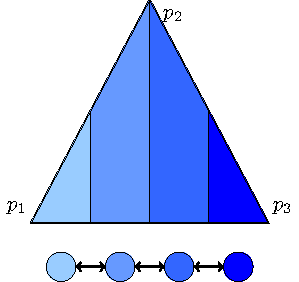
\includegraphics[width = 0.8\linewidth]{tikz/intersection-graph.pdf}
	\caption{Intersection graph for the [truncated] expected value property on outcomes $\Y = \{1,2,3\}$.}
	\end{minipage}
\hfill
	\begin{minipage}{0.48\linewidth}
	\centering
	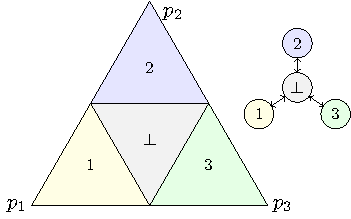
\includegraphics[width = 0.9\linewidth]{tikz/abstain-alpha-half.pdf}
	\caption{Intersection graph for the $\abstain{1/2}$ property on $\Y = \{1,2,3\}$.}
\end{minipage}
\end{figure}


\subsection{Proof approach: monotonicity}
\bo{Depending on space, we can give full definitions and proof sketches here, or less.}

The key idea of the proof is to define \emph{monotonicity} of a general property $g: \simplex \to 2^{R}$.
This generalizes orderability to the case where the report space $R$ is not necessarily finite
We show a finite property is orderable if and only if it is monotone.
From the definition of monotonicity, we are able to directly construct a polyhedral surrogate $L$, proving (1) $\implies$ (2) in Theorem \ref{thm:orderable-1-embed}.
The equivalence of embedding and polyhedral surrogates of \cite{finocchiaro2019embedding} (Theorem \ref{thm:embed-iff-poly}) gives (2) $\implies$ (3), and the fact that polyhedral functions are convex gives (3) $\implies$ (4).
Then, we show that monotone properties with report space $\reals$ are precisely those elicited by convex loss functions $L$.
This, along with a result that calibrated link functionss must also be in a sense ``ordered'', proves (4) $\implies$ (1).



%%%%%%%%%%%%%%%%%%%%%%%%%%%%%%%%%%%%%%%%%%%%%%%%%%%%%%%%%%%%%%%%
\section{Higher dimensions}\label{sec:d-dim}
\bo{blurb about the purpose of this section and the layout.}
\jessie{Taking a crack at it:}
\bo{Nice job!}
Our newfound understanding of the 1-dimensional embedding characterization leads us to realize that a large class of properties are not $1$-embeddable.
\cite{finocchiaro2019embedding} have shown a trivial upper bound that every property is $(n-1)$-embeddable, but it is an open question as to how tight we can get the bounds on embedding dimension.
Reducing embedding dimension significantly below $(n-1)$ can help provide a computational speedup in the optimization problem, which is a function of the surrogate loss dimension.
This is especially important as the number of possible outcomes $n$ grows large. 

Below, we generalize our characterization to $d$-embeddability for $d \geq 2$.
Having a finite number of embedding points and restricting to polyhedral functions allows us to study the subgradient sets of the loss at embedding points, which we formalize in Section~\ref{subsec:sub-sets}.
Using a general theory of polytopes, we can then present our general $d$-dimensional characterization in terms of optimality and monotonicity conditions.
In Section~\ref{subsec:opt-conditions}, we present a quadratic feasibility program in order to understand necessary conditions for $d$-embeddability by satisfying optimality conditions, yielding new lower bounds for embedding dimension in Corollary~\ref{cor:d-embeddable-char}.

\subsection{Setup: subgradient sets at embedding points.}\label{subsec:sub-sets}
%Recall that we have a loss function $\ell: \R \to \reals^{\Y}_{\geq 0}$, and for any prediction $r \in \R$ of the algorithm, we write $\gamma_r = \{ p : \inprod{p}{\ell(r)} \leq \inprod{p}{\ell(r')} (\forall r')\}$.
%We are interested in potential polyhedral surrogates $L: \reals^d \to \reals^{\Y}_{\geq 0}$.
%These are associated with embedding points, where $u_r \in \reals^d$ is linked back to the discrete prediction $r$.

Recall that if $\ell: \R \to \nonnegreals^{\Y}$ is embedded by $L: \reals^d \to \nonnegreals^{\Y}$, then each $r \in \R$ is embedded at some point $u_r \in \reals^d$.
In particular, $u_r$ must minimize $\inprod{p}{L(u)}$ if and only if $r$ minimizes $\inprod{p}{\ell(r')}$.

The key to our approach is to study as first-class objects the sets of all subgradients\footnote{Recall that a subgradient of e.g. the convex function $L(\cdot)_y: \reals^d \to \reals$ at a point $u$ is a vector $v \in \reals^d$ such that $L(u') \geq L(u) + \inprod{v}{u'-u}$ for all $u'$. The set of subgradients at $u$ is sometimes called the subdifferential.} of $L$ at these embedding points.
To settle the question of whether a consistent surrogate exists in $d$ dimensions, it surprisingly turns out to be necessary and sufficient to consider conditions on these sets alone.
In particular, we use heavily that a convex function is minimized at a point if and only if $\vec{0}$ is in its subgradient set at that point.

Therefore, we abstract to consider collections of sets $T^r_y$, which aspire to be the subgradient sets of a calibrated polyhedral surrogate $L(\cdot)_y$ at $u_r$.
Note that if $L(\cdot)_y$ is a polyhedral function on $\reals^d$, then all of its subgradient sets are (bounded) closed polytopes.\bo{cite}

\begin{definition}[$\T$, $\T^r$, $D(\T^r)$]
  We use the following notation for a collection of closed polytopes, with implicit parameter $d$: $\T = \{T^r_y \subseteq \reals^d : r \in \R, y \in \Y\}$.
  For each fixed $r$, we write $\T^r := \{T^r_y : y \in \Y\}$.

  Given a distribution $p \in \simplex$, we write the $p$-weighted Minkowski sum of $\T^r$ as
    \[ \oplus_p \T^r := \left\{ \sum_{y \in \Y} p(y) x^r_y ~\Big|~ x^r_1 \in T^r_1, \dots, x^r_y \in T^r_y \right\} , \]
  in other words, the Minkowski sum of the scaled sets $\{p(y) T^r_y : y \in \Y\}$.

  Finally, we associate with $\T^r$ a set of distributions $D(\T^r) = \{ p : \vec 0 \in \oplus_p \T^r\}$.
\end{definition}

The importance of the $p$-weighted Minkowski sum and of $D(\T^r)$ are that they capture the distributions $p$ for which $u_r$ minimizes expected loss, assuming that $\T$ correspond to some polyhedral $L$.
\begin{proposition} \label{prop:minkowski-0-opt}
  If $T^r_y$ is the subgradient set of each $L(u_r)_y$, then $D(\T^r)$ is the set of distributions $p \in \simplex$ for which the embedding point $u_r$ minimizes expected $L$-loss.
\end{proposition}
\begin{proof}
  Any convex function $f$ is minimized at $u$ if and only if $\vec 0$ is a subgradient of $f$ at $u$.
  Let $f(u) = \inprod{p}{L(u)}$.
  Then the subgradient set of $f$ at $u$ is $\oplus_p \T^r$.
  This follows from the basic properties that if $f_1,f_2$ are convex with subgradient sets $T_1,T_2$ at $u$, then $\alpha f_1$ has subgradient set $\alpha T_1$ and $f_1 + f_2$ has subgradient set $T_1 \oplus T_2$, the Minkowski sum.
  So $\vec 0$ is a subgradient of $\inprod{p}{L(u_r)}$ if and only if $\vec 0 \in \oplus_p \T^r$, which by definition occurs if and only if $p \in D(\T^r)$.
\end{proof}
This fact will be vital for characterizing when $\ell$ is correctly embedded by some $L$ whose subgradient sets are $\T$.
We leverage it next.

\subsection{General characterization}

We now give a general characterization of when a discrete loss $\ell$ can be embedded into $d$ dimensions, i.e. when a consistent polyhedral surrogate $L: \reals^d \to \reals^{\Y}_{\geq 0}$ exists.

Two conditions are required: \emph{optimality} and \emph{monotonicity}.
Optimality enforces that the surrogate is minimized precisely when and where it should be.
It says that for each discrete prediction $r$ and set of distributions $\gamma_r$ for which it is optimal, there exists a collection of polytopes $\T^r$ (presumably the subgradient sets of $L(u_r)_y$ for each $y$) realizing Proposition \ref{prop:minkowski-0-opt}.
Monotonicity says that these individual polytopes can actually be glued together to form the subgradients of some convex loss function $L$.

%\begin{definition}[Optimality of subgradients for a level set] \label{def:opt}
%  Given a collection of polytopes $\T^r = \{T_y^r \subseteq \reals^d : y \in \Y\}$ and a polytope $C \subseteq \simplex$, the \emph{optimality condition $\Opt(\T^r, C)$ holds} if $p \in C \iff \vec{0} \in \oplus_p T^r$.
%\end{definition}

\begin{theorem} \label{thm:general-char}
  Let $\ell: \R \to \reals_{\geq 0}^{\Y}$ be a discrete loss with, for each $r \in \R$, $\gamma_r = \{p : r \in \argmin_{r'} p \cdot \ell(r)\}$.
  Then $\ell$ is $d$-embeddable if and only if there exist polytopes $\T = \{T^r_y \subseteq \reals^d : r \in \R, y \in \Y\}$ such that both of the following hold:
  \begin{enumerate}
    \item (Optimality) For all $r \in \R$, we have $D(\T^r) = \gamma_r$.
    \item (Monotonicity) There exists an injective embedding function $\phi : \R \to \reals^d$ and loss functions $\{L_y : \reals^d \to \reals^\Y_{\geq 0}\}_{y \in \Y}$ such that for all $y \in \Y$ and $r \in \R$, we have $T^r_y = \partial L_y(\phi(r))$.
  \end{enumerate}
\end{theorem}
\begin{proof}
  TODO
\end{proof}


\subsection{Characterizing optimality}\label{subsec:opt-conditions}

We now investigate the optimality condition of Theorem \ref{thm:general-char}, for two purposes.
First, we aim to greatly narrow the search space for constructing low-dimensional surrogate loss functions for a given discrete loss.
The tools we construct in this section aid in this task by constraining or constructing feasible subgradient sets $\T^r$ given a level set $\gamma_r$.
Second, we wish to prove impossibilities, i.e. lower bounds on the embedding dimension of a given discrete loss (an apparently hard problem).

By dropping monotonicity from Theorem \ref{thm:general-char}, we obtain $|\R|$ independent optimality conditions, $D(\T^r) = \gamma_r$, that must be satisfied in order to have a $d$-dimensional embedding.
For upper bounds, one must construct a $\T^r$ satisfying $D(\T^r) = \gamma_r$ for all $r$ (and then turn to satisfying monotonicity).
For lower bounds, it suffices to prove nonexistence of any such $\T^r$, for any $r$.

To accomplish these, we construct a quadratic feasibility program (QFP, Definition \ref{def:qfp}) that takes as input a polytope $C \subseteq \simplex$ and a parameter $d \in \mathbb{N}$ and (roughly) attempts to construct $\T^r$.
We will prove the following main results.
\begin{theorem} \label{thm:opt-iff-qfp}
  Given a convex polytope $C \subseteq \simplex$, there exist polytopes $\T^r$ in $\reals^d$ such that $D(\T^r) = C$ if and only if there is a feasible solution to the QFP (Definition \ref{def:qfp}) with parameter $d$.
\end{theorem}

\begin{corollary}\label{cor:d-embeddable-char}
  If a discrete loss $\ell$ has any level set $C = \gamma_r = \{p : r \in \argmin_{r'} \inprod{p}{\ell(r')} \}$ for which the quadratic program is infeasible with parameter $d$, then $\ell$ is not $d$-embeddable.
\end{corollary}


\subsubsection{Feasibility program}

The feasibility program intuitively contains one set of necessary and one set of sufficient conditions.
The necessary conditions are derived from the representation of the polytope $C$ as an intersection of halfspaces.
The sufficient conditions are derived from its dual representation as a convex hull of vertices.

The variables are a set of normal vectors $\{v_i \in \reals^d : i \in [k]\}$ and a set of vertices $\{x^j_y \in \reals^d : j \in [\ell], y \in \Y\}$.
These correspond to a (possibly relaxed) halfspace representation and (possibly incomplete) vertex representation of the subgradient polytopes $\T^r$.

\begin{definition}[Quadratic Feasibility Program] \label{def:qfp} ~ \\
  \indent \textbf{Parameter:} $d \in \mathbb{N}$.

  \textbf{Given:} a polytope $C = \{p \in \simplex : Bp \geq \vec 0\} = \conv(\{p^1, \ldots, p^\ell\}) \subseteq \simplex$, where $B \in \reals^{k \times n}$ has a minimum number of rows.

  \textbf{Variables:} a matrix $V \in \reals^{k \times d}$, each row representing a normal vector; and a collection of matrices $X^1,\ldots,X^{\ell} \in \reals^{d \times n}$, with $X^j$ intuitively corresponding to $p^j$ with columns $x^j_y$ representing witness points.

  \textbf{Constraints:}
    \begin{align}
      V X^j                     &\leq B    & \text{(pointwise, $\forall j \in [\ell]$)}  \label{eqn:qp-constr-1} \\
      \sum_{y=1}^n p^j(y) x^j_y &= \vec 0  & \text{($\forall j \in [\ell]$)}    \label{eqn:qp-constr-2} 
    \end{align}
\end{definition}

The feasibility program can be viewed as a low-rank matrix problem, namely: do there exist a set of rank-$d$ matrices that are pointwise dominated by $B$, sharing the left factor $V$, whose right factors $X^j$ respectively satisfy a subspace constraint?
We will see \bo{in which section?} that for the important example of abstain loss, the constraints simplify into a more pure low-rank matrix problem.
In particular, for $d=n-1$ a solution always exists (e.g. \bo{cite}), found by taking the convex conjugate of the Bayes risk of $\ell$ \bo{and then what?}.


\subsubsection{Developing the proof}

To prove Theorem \ref{thm:opt-iff-qfp}, it is useful to develop a less-constructive intermediate characterization of when $D(\T^r) = C$.
The following condition formalizes a necessary condition on $\T^r$ in terms of the halfspace representation of $C$; the subsequent one formalizes a sufficient condition using the vertex representation.


\begin{condition}[Halfspace condition]\label{cond:H-condition}
	A collection of polytopes $\T^r$ and a polytope $C$ in the simplex defined by $C = \{p \in \simplex : Bp \geq \vec 0\}$ \emph{satisfy the halfspace condition} if there exist $v_1, \ldots, v_k \in \reals^d$ such that, for all $i \in [k]$ and $y \in \Y$, for all $x \in T^r_y$, we have $\inprod{v_i}{x} \leq B_{iy}$.
\end{condition}
\begin{condition}[Vertex condition]\label{cond:V-condition}
	A collection of polytopes $\T^r$ and a polytope $C$ in the simplex defined by $C = \conv(\{p^1, \ldots, p^\ell\})$ \emph{satisfy the vertex condition} if for all $j \in [\ell]$, $0 \in \oplus_{p^j} \T^r$. %% Equivalent: there exist $\{x_{jy} \in T_y : j \in [\ell]\}$ such that, for all $j \in [\ell]$, $\sum_{y \in \Y} p^j_y x_{jy} = \vec 0$.
\end{condition}

Useful lemmas:
\begin{lemma} \label{lemma:D-polytope}
  For any $\T^r$, $D(\T^r)$ is a polytope (in particular, is convex).
\end{lemma}
\begin{proof}
   Recall by definition, the notation $\oplus_p \T^r = \{\sum_y p(y) x^r_y : x^r_y \in T^r_y (\forall y)\}$.
   Each $T^r_y$ is a polytope, so $p(y) T^r_y$ is a polytope.
   The Minkowski sum of polytopes is a polytope, so $\oplus_p \T^r$ is a polytope.
  \bo{TODO}
\end{proof}
\begin{lemma}  \label{lemma:minkowski-support}
  Given polytopes $\T^r$, there exists a finite set of normal vectors $w_1,\ldots,w_K \in \reals^d$ such that, for all $p \in \simplex$, $\oplus_p \T^r = \{x : \inprod{w_i}{x} \leq \sum_{y \in \Y} p(y) \max_{x \in T^r_y} \inprod{w_i}{x} \}$.
\end{lemma}
\begin{proof}
   For each $p$, $\oplus_p \T^r$ is a polytope.

  \bo{TODO: it turns out that $p$ doesn't matter, only its support; and there are only finitely many possible supports (or even better, the normals that are complete for the uniform minkowski sum turn out to be complete for all other $p$-combinations).}
\end{proof}
\begin{lemma} \label{lemma:E-to-B}
  Let $C = \{p : Bp \geq \vec 0 \}$ where $B$ has the minimum possible number of rows to capture $C$, and suppose $C = \{p : Ep \geq \vec 0 \}$.
  Then for each row in $B$ there is some (unique) row in $E$ that is equal to $\alpha B$ for some positive $\alpha$.
\end{lemma}
\begin{proof}
  \bo{? Cite} \jessie{Is left as an exercise in the following text:} \cite[Exercise 2.15]{ziegler2012lectures}
\end{proof}


\begin{theorem} \label{thm:vertex-halfspace-opt}
  Let the polytopes $\T^r = \{T^r_y \subseteq \reals^d : y \in \Y\}$ and $C$ be given, with $C = \conv(\{p^1,\ldots,p^{\ell}\}) = \{p: Bp \geq \vec 0\}$ for $B \in \reals^{k \times n}$.
  We have $D(\T^r) = C$ if and only if both the halfspace and vertex conditions hold.
\end{theorem}
\begin{proof}
  ($\implies$)
  Suppose $D(\T^r) = C$.
  First, we note that the vertex condition is immediate: For all $j \in [\ell]$, $p^j \in C$ which gives $p^j \in D(\T^r)$.
  To show the halfspace condition is satisfied, we first construct a matrix $E$ such that $Ep \geq 0 \iff Bp \geq 0$, then use this construction to pick out the necessary vectors $v_1,\dots,v_k$.

  By Lemma \ref{lemma:minkowski-support}, there is a finite collection of vectors $w_1,\dots,w_{K} \in \reals^d$ and such that $\vec 0 \in \oplus_p \T^r$ if and only if, for all $w_i$, $\sum_y p(y) \max_{x \in T^r_y} \inprod{w_i}{x} \geq 0$.
  Hence, each vector $w_i$ generates a row of a matrix $E \in \reals^{K \times n}$ with $E_{iy} = \max_{x \in T^r_y} \inprod{w_i}{x}$, and we have $p \in D(\T^r) \iff Ep \geq 0$.
  By assumption of $D(\T^r) = C$, then, we have $Ep \geq 0 \iff Bp \geq 0$.
  By Lemma \ref{lemma:E-to-B}, because $B$ has the minimum possible number of rows, each row of $B$ appears (scaled by some positive constant) as a different row of $E$. Taking the collection of $w_i$ corresponding to these rows and rescaling them by that positive constant, we get a collection of $k$ vectors that we can rename $v_1,\ldots,v_k \in \reals^d$, with $\max_{x \in T^r_y} \inprod{v_i}{x} = B_{iy}$, hence the halfspace condition is satisfied.

  ($\impliedby$)
  Suppose Conditions \ref{cond:H-condition} and \ref{cond:V-condition} hold.
  Then by the vertex condition, $p^j \in D(\T^r)$ for all $j \in [\ell]$.
  Because $D(\T^r)$ is convex (Lemma \ref{lemma:D-polytope}), this implies $C \subseteq D(\T^r)$.
  To show $D(\T^r) \subseteq C$, let $p \in D(\T^r)$; by definition, $0 \in \oplus_p \T^r$.
  Then in particular for each vector $v_1,\ldots,v_k$ guaranteed by the halfspace condition, we have
  \begin{align*}
    0 &\leq \max_{x \in \oplus_p \T^r} \inprod{v}{x}  \\
      &=    \sum_{y \in \Y} p(y) \max_{x \in T^r_y} \inprod{v_i}{x}  \\
      &\leq \sum_{y \in \Y} p(y) B_{iy} .
  \end{align*}
  This proves $Bp \geq 0$, so $p \in C$.
\end{proof}

Given this characterization, we prove the main result on when a solution to the quadratic program exists.
\bo{Should note that the program's solution does give candidates $\T^r$, although their usefulness is unclear...}
\bo{Actually, I guess one could run this, then use monotonicity to add constraints and find the next subgradient sets, etc.}

\begin{proof}[Proof of Theorem \ref{thm:opt-iff-qfp}]
    By Theorem \ref{thm:vertex-halfspace-opt}, it suffices to show that $\T^r$ satisfying the halfspace and vertex conditions exist if and only if the program is feasible.

  ($\implies$) 
  By the vertex condition, for each $j \in [\ell]$, there exist witnesses $\{x^j_y \in T^r_y : y \in \Y\}$ satisfying the second constraint of the quadratic program (Inequality \ref{eqn:qp-constr-2}).
  By the halfspace condition, there exist normals $v_1, \dots, v_k$ such that, for all $i$, for all $x \in T^r_y$, $\inprod{v_i}{x} \leq B_{iy}$; in particular, this applies to the above witnesses $x^j_y \in T^r_y$.
  Collecting $v_1,\dots,v_k$ as the columns of $V$, this shows that the first constraint (Inequality \ref{eqn:qp-constr-1}) is satisfied.

  \bigskip
  ($\impliedby$)
  We construct $T^r_y = \conv(\{x^1_y, \ldots, x^{\ell}_y\})$.
  The second constraint of the quadratic program immediately implies the vertex condition.
  Taking $v_1,\dots,v_k$ as the columns of $V$, the first constraint implies that for each $x^j_y$, we have $\inprod{v_i}{x^j_y} \leq B_{iy}$ for all $i,j,y$.
  Any point $x \in T^r_y$ is a convex combination of $x^1_y,\ldots,x^{\ell}_y$, so it satisfies $\inprod{v_i}{x} \leq B_{iy}$.
  This implies the halfspace condition.  % Bo: QED
\end{proof}

  


%%%%%%%%%%%%%%%%%%%%%%%%%%%%%%%%%%%%%%%%%%%%%%%%%%%%%%%%%%%%%%%%
\section{Examples}\label{sec:examples}
\subsection{Abstain property, $\alpha \leq 1/2$}\label{subsec:example-abstain}
One classification-like problem that is of particular interest is the abstain property, elicited by the loss $\ellabs{1/2}$ given in Equation~\ref{eq:abstain}.
The property $\abstain{\alpha}$ can be verified:
\begin{equation}\label{eq:abstain-prop}
     \abstain{\alpha} = \begin{cases}
     \argmax_{y \in \Y} p(y) & \max_y p(y) \geq 1 - \alpha\\ 
     \bot & \text{otherwise}
     \end{cases}~.~
\end{equation}

\cite{ramaswamy2018consistent} study the abstain property in great length, presenting a $\ceil {\log_2(n)}$ dimension embedding of the abstain property.
However, it is unclear if this bound is tight, as the previously studied lower bounds of~\cite{ramaswamy2016convex} do not work well for this property, failing to give anything tighter than the trivial $1 \leq \elicembed(\abstain{\alpha})$ for $\alpha \leq 1/2$.

With our $1$-dimensional characterization, we already observe a tighter lower bound.
\begin{proposition}
	For $n \geq 3$ and $\alpha \leq 1/2$, we have $\elicembed(\abstain{1/2}) \geq 2$.
\end{proposition}
\begin{proof}
	Consider the intersection graph of $\gamma := \abstain{\alpha}$: the node associated with $\gamma_\bot$ has $n$ edges, and since we assume $n \geq 3$, we fail to observe the requirement that every node of the intersection graph has degree at most $2$.
\end{proof}

\begin{proposition}
	$\gamma := \abstain{1/2}$ with $n=5$ is not $2$-embeddable.
\end{proposition}
\begin{proof}
  We use the results from Section~\ref{sec:d-dim} and show that the optimality condition is not met for the level set $\gamma_\bot$.
  First, we represent the cell $\gamma_\bot = \{p \in \simplex : Bp \geq \vec 0\} = \conv(\{(1/2, 1/2, 0,0,0), \ldots, (0,0,0,1/2, 1/2)\})$, where $B = \ones \ones^T - 2I_5 \in \reals^{5 \times 5}$ has entry $-1$ on the diagonal, and entry $1$ everywhere else.
	
  We make an argument on the permissible angles between normals $v_1, \ldots, v_5$ in $\reals^2$ and show there is no feasible solution to the QFP in Definition~\ref{def:qfp}.
  In particular, we argue that for any cone strictly $ < 180^\circ$, we can have no more than two vectors $v_i$ and $v_j$; otherwise we yield a contradiction.
  
  Without loss of generality, we let $v_1 = (0,1)$, and have $v_2$ with $\|v_2\|^2 \leq \|v_1\|^2$ and the angle $\theta_{12} < 180^\circ$ the angle between $v_1$ and $v_2$.
  
  We then have the feasible regions $F_y = \{x \in \reals^2 : \inprod{v_i} {x} \leq B_{iy} \; \forall i\}$, which means to this point, we have $F_1 = \{x \in \reals^2 : \inprod{v_1}{x} \leq -1 \text{ and } \inprod{v_2}{x} \leq 1 \}$, and $F_2 = \{x \in \reals^2 : \inprod{v_1}{x} \leq 1 \text{ and } \inprod{v_2}{x} \leq -1 \}$.
  By requirement of the existence of a set of witnesses for the distribution $(1/2, 1/2, 0,0,0)$, we must have some $x^{12}_1 \in F_1$ and $x^{12}_2 \in F_2$ so that $x^{12}_1 = -x^{12}_2$ in order for $\vec 0$ to be in the Minkowski sum.
  In particular, we know that, since $\theta_{12} < 180^\circ$, $x^{12}_1$ and $x^{12}_2$ are unique given $v_1$ and $v_2$.
  
  We then want to show that we cannot add a $v_3$ such that $\max(\theta_{12}, \theta_{13}, \theta_{23}) < 180^\circ$ without yielding a contradiction, which then gives our result, as any arrangement of $5$ normals in $\reals^2$ must have some cone that is less than $180^\circ$ containing three normals.

  In general, observe that $x^{12}_1$ and $x^{13}_1$ must both be on the line $\inprod{v_1}{x} = -1$. \jessie{More detail}  
  Therefore, our three cases proceed as follows: $(i.) \|x^{13}_1\| > \|x^{12}_1\|$, $(ii.) \|x^{13}_1\| = \|x^{12}_1\|$, and $(iii.) \|x^{12}_1\| > \|x^{13}_1\|$.
  As the labels on normals $v_2$ and $v_3$ (and therefore, the respective witnesses) are arbitrary, it suffices to just show cases $(i.)$ and $(ii.)$.
  
  \begin{enumerate}
  \item [$(i.)$] First, suppose $\|x^{13}_1\| < \|x^{12}_1\|$.
  This in turn implies that $\|v_3\| > \|v_2\|$ since both witnesses are on the line $\inprod{v_1}{x^{1i}_1} = -1$.
  Consider that in order for $x^{12}_1 \in F_1$, we must have both $\inprod{v_2}{x^{12}_1} = 1$ and $\inprod{v_3}{x^{12}_1} \leq 1$.
    \begin{align*}
    \inprod{v_2}{x^{12}_1} = 1 &\iff \|v_2\| \cos(\theta(v_2, x^{12}_1)) = \frac 1 {\|x^{12}_2\|}\\
    \inprod{v_3}{x^{12}_1} \leq 1 &\iff \|v_3\| \cos(\theta(v_3, x^{12}_1)) \leq \frac 1 {\|x^{12}_2\|}\\
\implies \|v_3\| \cos(\theta(v_3, x^{12}_1)) &\leq \|v_2\| \cos(\theta(v_2, x^{12}_1))\\
\implies 1 < \frac{\|v_3\|}{\|v_2\|} &\leq \frac{\cos(\theta(v_2, x^{12}_1))}{\cos(\theta(v_3, x^{12}_1))}\\
\implies \theta(v_3, x^{12}_1) &> \theta(v_2, x^{12}_1)\\
\implies \theta_{13} < \theta_{12}
    \end{align*}
    This yields a contradiction, as we must have $\theta_{12} < \theta_{13}$ in order to have $\inprod{v_3}{x^{13}_1} = \inprod{v_2}{x^{12}_1} = 1$.
    Therefore, we conclude that we cannot have $\|x^{12}_1\| > \|x^{13}\|$.
  	\item [$(ii.)$] Suppose that we have $\|x^{12}_1\| = \|x^{13}_1\|$.
  	As both witnesses are on the same halfspace $\{x : \inprod{v_1}{x} = -1\}$, we must have $x^{12}_1 = x^{13}_1$.
  	
  \end{enumerate}  
  
%  We do this by arguing that in all three cases of the argmax, we either restrict $F_1$ so that $x_1 \not \in F_1$, restrict $F_2$ so that $x_2 \not \in F_2$, or have $x_3 \not \in F_3$.
%  We merge the latter two cases without loss of generality as we can relabel these normals pretty easily because of the structure of $B$.
%

%  
%  \begin{enumerate}
%  	\item [$\theta_{23} = \argmax$] 
%  	Since $\theta_{23} < 180^\circ$ and $v_1$ is in the middle of $v_2$ and $v_3$, we have that $x^{12}_1 \neq x^{13}_1$.
%  	Without loss of generality, suppose $\|v_2\|^2 \leq \|v_3\|^2$.
%  	Then we claim that $x^{13}_1 \not \in F_1$, since we have $x^{13}_1 = \{x : \inprod{v_1}{x} = -1 \text{ and } \inprod{v_3}{x} = 1\}$.
%  \end{enumerate}
  
\end{proof}
\begin{proof}[Matrix rank proof]
  We can understand the QFP given in Section~\ref{sec:d-dim} for $\abstain{1/2}$ as a matrix rank problem.
  \jessie{Fill in explanation}
  
  With $n=4$, we observe the following matrix rank problem:
  \[
  \begin{bmatrix}
  	-1 & -1 & -1 & \cdot & \cdot & \cdot \\
  	1 & \cdot & \cdot & -1 & -1 & \cdot \\
  	\cdot & 1 & \cdot & 1 & \cdot & -1 \\
  	\cdot & \cdot & 1 & \cdot & 1 & 1 \\
  \end{bmatrix}
  \]
  
  Since this matrix is a submatrix of the matrix rank problem for $n=5$, any solution of this above problem must also be a solution in the large matrix given below.
  
  \[
  \begin{bmatrix}
  {\color{red} -1} & {\color{red} -1} & {\color{red} -1} & {\color{red} \cdot} & {\color{red} \cdot} & {\color{red} \cdot} & -1 & \cdot & \cdot & \cdot \\
  {\color{red} 1} & {\color{red} \cdot} & {\color{red} \cdot} & {\color{red} -1} & {\color{red} -1} & {\color{red} \cdot} & \cdot & -1 & \cdot & \cdot \\
  {\color{red} \cdot} & {\color{red} 1} & {\color{red} \cdot} & {\color{red} 1} & {\color{red} \cdot} & {\color{red} -1} & \cdot & \cdot & -1 & \cdot \\
  {\color{red} \cdot} & {\color{red} \cdot} & {\color{red} 1} & {\color{red} \cdot} & {\color{red} 1} & {\color{red} 1} & \cdot & \cdot & \cdot & -1 \\
  \cdot & \cdot & \cdot & \cdot & \cdot & \cdot & 1 & 1 & 1 & 1\\
  \end{bmatrix}
  \]
  
  In characterizing the solutions to the smaller matrix rank problem, let us establish the linear equality of the first two rows and second two rows.
  (Note that any combination of row pairs works without loss of generality.)
  The first column containing $[-1 \; 1]^T$ implies that we must have the two rows being the negation of each other, and similarly for the third and fourth rows with the final column.
  This gives a matrix of rank 2 as follows:
  \[
    \begin{bmatrix}
  -1 & -1 & -1 & 1 & 1 & a \\
  1 & 1 & 1 & -1 & -1 & -a \\
  b & 1 & -1 & 1 & -1 & -1 \\
  -b & -1 & 1 & -1 & 1 & 1 \\
  \end{bmatrix}
  \] with $a, b \in [-1,1]$.
  One can verify that we cannot obtain a matrix of rank $1$, regardless of the choice of $a$ and $b$.
  Plugging in this solution set into the larger matrix yields
  \[
  \begin{bmatrix}
  {\color{red} -1} & {\color{red} -1} & {\color{red} -1} & {\color{red} 1} & {\color{red} 1} & {\color{red} a} & -1 & \cdot & \cdot & \cdot \\
  {\color{red} 1} & {\color{red} 1} & {\color{red} 1} & {\color{red} -1} & {\color{red} -1} & {\color{red} a} & \cdot & -1 & \cdot & \cdot \\
  {\color{red} b} & {\color{red} 1} & {\color{red} -1} & {\color{red} 1} & {\color{red} -1} & {\color{red} -1} & \cdot & \cdot & -1 & \cdot \\
  {\color{red} -b} & {\color{red} -1} & {\color{red} 1} & {\color{red} -1} & {\color{red} 1} & {\color{red} 1} & \cdot & \cdot & \cdot & -1 \\
  \cdot & \cdot & \cdot & \cdot & \cdot & \cdot & 1 & 1 & 1 & 1\\
  \end{bmatrix}
  \]
  
  In order for the $5^{th}$ row to be linearly dependent with the first two rows, we must have $r_5 = -r_1$ by the column $c_7$, and $r_5 = r_2$ by column $c_8$, yielding a contradiction.
  Similarly, we cannot establish linear independence with the last two rows because of restrictions imposed by columns $c_9$ and $c_{10}$.
  Therefore, the matrix completion problem given above has no solution of rank 3, and we conclude that $\abstain{1/2}$ is not $2$-embeddable with $n=5$.
\end{proof}


\newpage
% Acknowledgments---Will not appear in anonymized version
\acks{JF- Need that GRFP acknowledgement}

\bibliography{diss,extra}

\newpage
\appendix

\section{Additional proofs}


\section{Feasible subspace dimension}


\end{document}

%%% Local Variables:
%%% mode: latex
%%% TeX-master: t
%%% End:
